\section{UML-Diagram} % (fold)
\label{sec:uml_diagram}

\begin{figure}[h]
    \centering
    \begin{subfigure}{0.49\textwidth}
        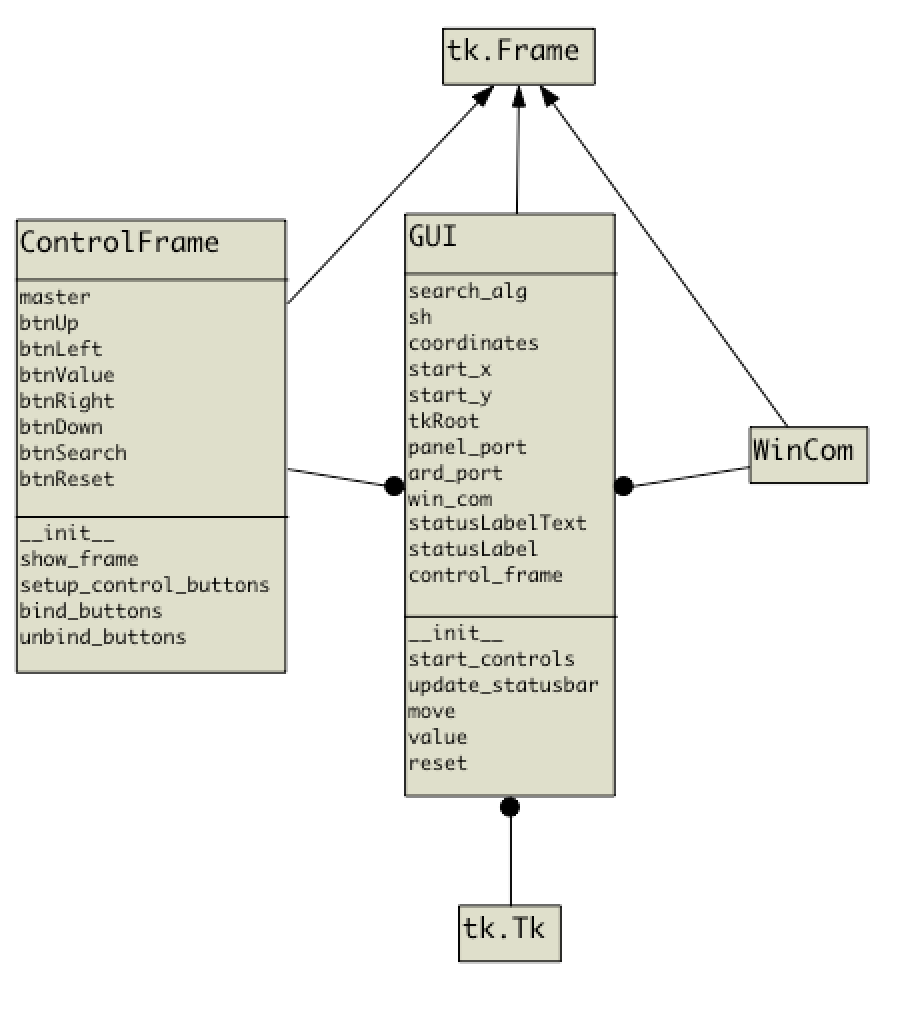
\includegraphics[width=\textwidth]{res/img/GUI_uml}
        \caption{Översikt av det grafiska gränssnittet}
    \end{subfigure}
    \begin{subfigure}{0.49\textwidth}
        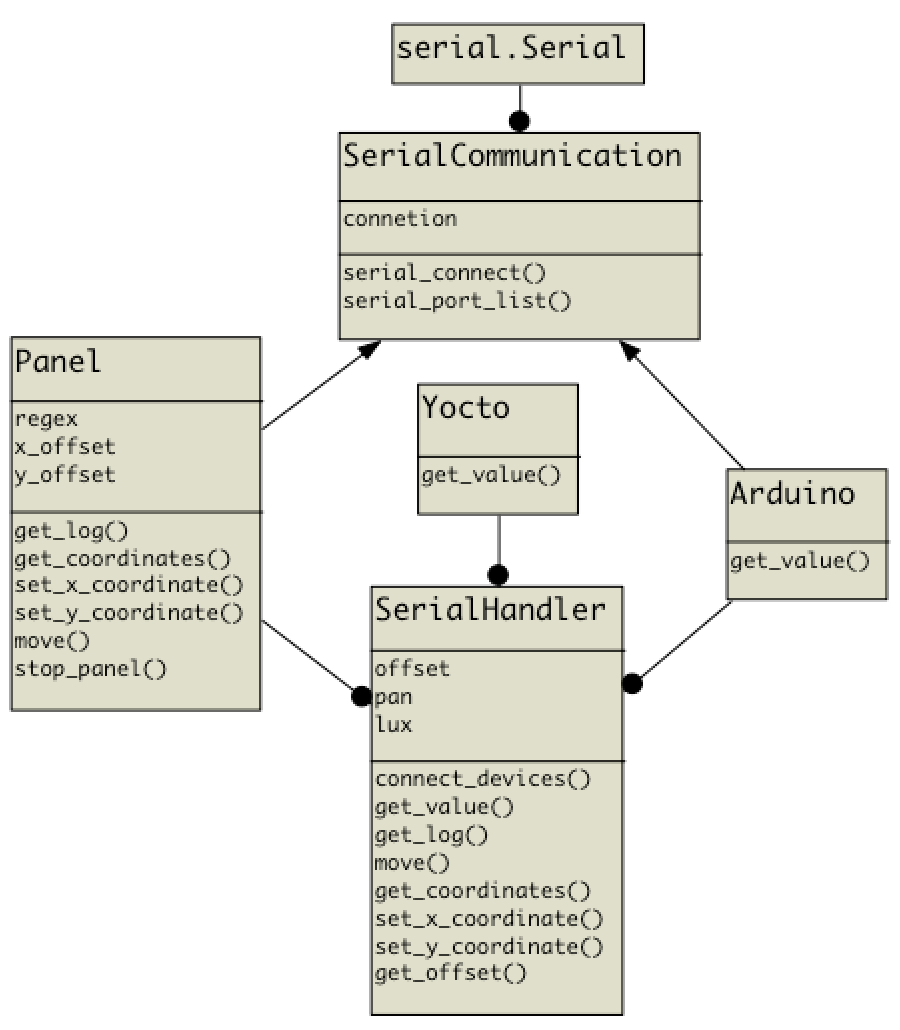
\includegraphics[width=\textwidth]{res/img/serial_uml}
        \caption{Översikt av den seriella kommunikationen}
    \end{subfigure}
\end{figure}
\vspace{20mm}
\begin{minipage}[l]{0.49\textwidth}
    \vspace*{2em}
    \centering
        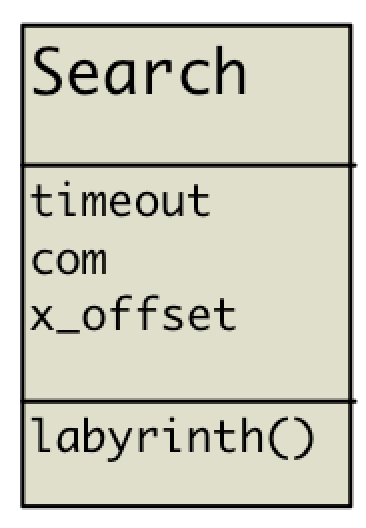
\includegraphics[scale=0.25]{res/img/search_uml} \\
        \vspace*{3.7em}
        (c) Klassen som håller kalibreringsalgoritmen. \\ Ärver inte av andra
\end{minipage}
\begin{minipage}[l]{0.49\textwidth}
    \vspace{-3.5em}
        \begin{verbatim}
# Main.py
from search import Search
from serial_handler import SerialHandler
from gui.gui import GUI
import sys

def is_windows():
    return sys.platform.startswith('win')

sh = SerialHandler()
search = Search(sh)
GUI(sh, search, windows=is_windows())
\end{verbatim}
        \centering
        (d) Skriptet som initierar applikationen.
\end{minipage}

\vfill
\begin{center}
Fullständig källkod finns att tillgå på: \texttt{github.com/MrAkergren/calibration}
\end{center}

% section uml_diagram (end)